\documentclass[a4paper,11pt,onecolumn,twoside]{article}

\usepackage{xeCJK}       % 使用XeLaTeX编译
\usepackage{CJK}
\usepackage{fancyhdr}
\usepackage{amsmath,amsfonts,amssymb,graphicx}
\usepackage{graphics}
\usepackage{subfigure}
\usepackage{indentfirst}
\usepackage{bm}          % 公式中的粗体字符(用命令\boldsymbol)
\usepackage{multicol}    % Two cols
\usepackage{multirow}    %
\usepackage{abstract}

% For MATLAB Code
\usepackage{listings}
\usepackage[T1]{fontenc}
\usepackage{bigfoot}    % to allow verbatim in footnote
\usepackage[numbered,framed]{matlab-prettifier}



% 下面的命令重定义页面边距

\addtolength{\topmargin}{-54pt}
\setlength{\oddsidemargin}{-0.9cm}  % 3.17cm - 1 inch
\setlength{\evensidemargin}{\oddsidemargin}
\setlength{\textwidth}{17.00cm}
\setlength{\textheight}{24.00cm}    % 24.62
\setCJKmainfont[BoldFont=SimHei,ItalicFont={[stkaiti.ttf]}]{SimSun}

\newfontfamily\kai{STKaiti}          % 楷体
\newfontfamily\hei{SimHei}           % 黑体


\renewcommand{\baselinestretch}{1.1} %定义行间距
\renewcommand{\multirowsetup}{\centering}
\parindent 22pt %重新定义缩进长度



\title{\huge{DSP第二次大作业报告:\\IIR数字滤波器设计}
\thanks{本文为 \textbf{数字信号处理} 课程第二次大作业报告,提交日期为2017.6.14.}}
\author{杨宇喆 \\[2pt]
\normalsize
1400012996 \qquad yuzhe.yang@pku.edu.cn
\\[2pt]}

\date{}  % 这一行用来去掉默认的日期显示


% ==================================首页页眉页脚定义

\fancypagestyle{plain}{
\fancyhf{}
\lhead{School of EECS\\
\scriptsize{Peking University}}
\chead{\centering{DSP第二次大作业报告\\
\scriptsize{\textbf{Report of Second Project, Digital Signal Processing}}}}
\rhead{1400012996\\
\scriptsize{yuzhe.yang@pku.edu.cn}}
\lfoot{}
\cfoot{}
\rfoot{}}



% ================================R,C,L分别代表左中右,O,E代表奇偶页

\pagestyle{fancy}
\fancyhf{}
\fancyhead[R]{杨宇喆 1400012996}
\fancyhead[C]{DSP第二次大作业报告:IIR数字滤波器设计}
\fancyhead[L]{\thepage}
\lfoot{}
\cfoot{}
\rfoot{}


\newenvironment{figurehere}
  {\def\@captype{figure}}
  {}
\makeatother



\begin{document}

\newcommand{\supercite}[1]{\textsuperscript{\cite{#1}}}

\maketitle

%  恢复正文页边距
\setlength{\oddsidemargin}{-.5cm}  % 3.17cm - 1 inch
\setlength{\evensidemargin}{\oddsidemargin}
\setlength{\textwidth}{17.00cm}
%\CJKfamily{song}

% one side


\iffalse
% ===================================插入图片格式 //暂时无标题
\begin{center}
    \includegraphics[width=1\textwidth]{test.jpg}
\end{center}

% ===================================插入Matlab代码格式,参考matlab-prettifier文档
\begin{lstlisting}[style=Matlab-editor,
                   basicstyle=\mlttfamily,
                   caption={My 1st Code}, label=code1]
while `\mlplaceholder{condition}`
    if `\mlplaceholder{something-bad-happens}`
        break
    else
    % do something useful
    end
end
\end{lstlisting}
\fi


\section{实验原理概述}

\subsection{$IIR$数字滤波器}
数字滤波器是对数字信号进行滤波处理以得到期望的响应特性的离散时间系统~\supercite{wiki}。作为一种电子滤波器,数字滤波器与完全工作在模拟信号域的模拟滤波器不同。数字滤波器工作在数字信号域,它处理的对象是经由采样器件将模拟信号转换而得到的数字信号。

线性移不变的数字滤波器包括无限长脉冲响应滤波器~(IIR滤波器)和有限长脉冲响应滤波器~(FIR滤波器)两种。这两种滤波器的系统函数可以统一以$Z$变换表示为~\supercite{textbook}:

\begin{equation}
H(z) = \frac{B(z)}{A(z)} = \frac{b_0+b_1 z^{-1}+b_2 z^{-2}+\cdots +b_N z^{-N}}{1+a_1 z^{-1}+a_2 z^{-2}+\cdots +a_M z^{-M}}.
\end{equation}
当$M\geq 1$时,$M$就是IIR滤波器的阶数,表示系统中反馈环的个数。由于反馈的存在,IIR滤波器的脉冲响应为无限长,因此得名~\supercite{wikifft}。

IIR滤波器的优点在于,其设计可以直接利用模拟滤波器设计的成果,因为模拟滤波器本身就是无限长冲激响应的。通常IIR滤波器设计的过程如下:首先根据滤波器参数要求设计对应的模拟滤波器(如巴特沃斯滤波器、切比雪夫滤波器等等),然后通过映射(如脉冲响应不变法、双线性映射等等)将模拟滤波器变换为数字滤波器,从而决定IIR滤波器的参数~\supercite{course1}。IIR滤波器的重大缺点在于,由于存在反馈其稳定性不能得到保证。另外,反馈还使IIR滤波器的数字运算可能溢出。

\subsection{$IIR$数字滤波器设计方法}
在本实验中,我们才用间接设计法来设计IIR数字滤波器,即先通过设计相对应指标的模拟滤波器,后经过频率域映射变换得到相应的数字滤波器。其设计过程如下~\supercite{course3}:
\begin{enumerate}
\item 确定数字滤波器指标;
\item 将数字滤波器指标转换为相应的模拟滤波器指标;
\item 设计满足指标要求的过渡模拟函数$H(s)$;
\item 设将过渡模拟函数$H(s)$转换为数字滤波器$H(z)$。
\end{enumerate}

把模拟滤波器$H_a(s)$转换为数字滤波器$H(z)$的实质是,用一种从$s$平面到$z$平面的映射函数将$H_a(s)$转换$H(z)$。对这种映射函数的要求是:因果稳定的模拟滤波器转换为数字滤波器$H(z)$后仍然稳定;数字滤波器$H(z)$的频率响应特性能够近似模仿数字滤波器$H_a(s)$的片段常数频率响应特性。常用的模拟--数字滤波器变换方法有:脉冲响应不变法和双线性变换法。

\subsubsection{脉冲响应不变法}
冲激响应不变法的思想是:使数字滤波器的单位冲激响应序列$h(n)$与模拟滤波器的单位冲激响应$h_a(t)$在抽样点上相等~(时域模拟)~\supercite{course3}。
\begin{equation}
h(n) = \hat{h}_a(nT) = \hat{h}_a(t) \big|_{t=nT}
\end{equation}
对于其频率响应,我们可以推导出
\begin{equation}
H(e^{j\omega})\big|_{\omega = \Omega T} = \frac{1}{T} \sum_{k= - \infty}^{\infty} H_a\big( j\Omega -jk\frac{2\pi}{T} \big),
\end{equation}
其中
\begin{equation}
z = e^{j\omega}, \quad \ s = j\Omega.
\end{equation}

冲激响应不变法的特点和问题分别有~\supercite{course4}:
\begin{enumerate}
\item 该方法使数字滤波器的冲激响应完全模仿模拟滤波器的冲激响应,因此时域逼近良好;
\item $\omega = \Omega T$为一线性关系,可以保持相位响应的线性度;
\item 当$H_a(s)$便于部分分式分解时,该方法设计简单明了;
\item 易产生频率混叠失真,该方法只能用于限带的模拟低通滤波器,对于高通和带阻滤波器,不宜用此法设计。
\end{enumerate}

\subsubsection{双线性变换法}
由于脉冲响应不变法存在缺点,即因为$s$域到$z$域是多值映射,映射关系不是单值对应,由于实际的模拟滤波器都不是完全带限的,所以会产生混叠失真。
而且脉冲响应不变法只适合频率响应在高频处单调递减的模拟原型滤波器,因此其应用范围受到限制。

双线性变换法的主要目的是避免多值映射,原理是先将$s$平面进行压缩至$s_1$平面,再将压缩的$s_1$平面向$z$平面进行单值映射,从而解决混叠的问题。其频率对应关系则变为
\begin{equation}
\Omega = c \tan (\frac{\Omega_1 T}{2}) = c \tan (\frac{\omega}{2}).
\end{equation}

双线性变换法的优缺点分别是~\supercite{course3}:
\begin{enumerate}
\item 模拟频率域数字频率是单值对应关系,避免了冲激响应不变法的混叠失真;
\item 映射函数在频率零点附近有较好的线性近似,但随着$\Omega$的增加,$\Omega$和$\omega$之间便存在着严重的非线性关系可能产生严重的非线性失真。
\end{enumerate}



\section{实验过程及数据}

\subsection{源信号录制}
在本实验中,我采用录制自己的声音作为源信号~\supercite{ta}。其中,具体操作是:以$8kHz$采样频率直接在$Matlab$中录制自己的声音,长度为$5s$, 运行平台是$Windows$ 10 $64bit$,$Matlab\ R2014a$,采用的函数是自带的录制函数$audiorecorder$。在录制完成后我将其保存于$myrecord.mat$文件中,并直接在文件中调用。

录制的音频时域波形和频域谱函数分别如图1和图2所示。
\begin{center}
    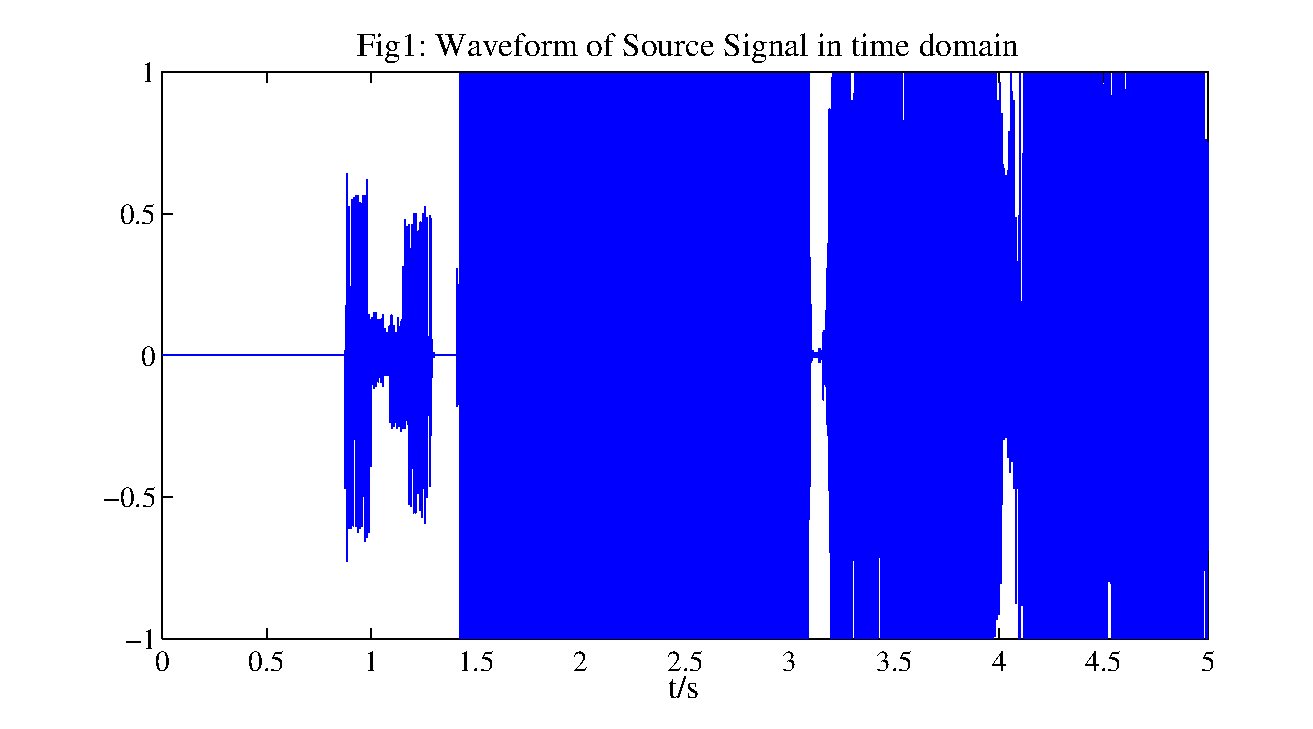
\includegraphics[width=1\textwidth]{fig1.eps}
\end{center}
\begin{center}
    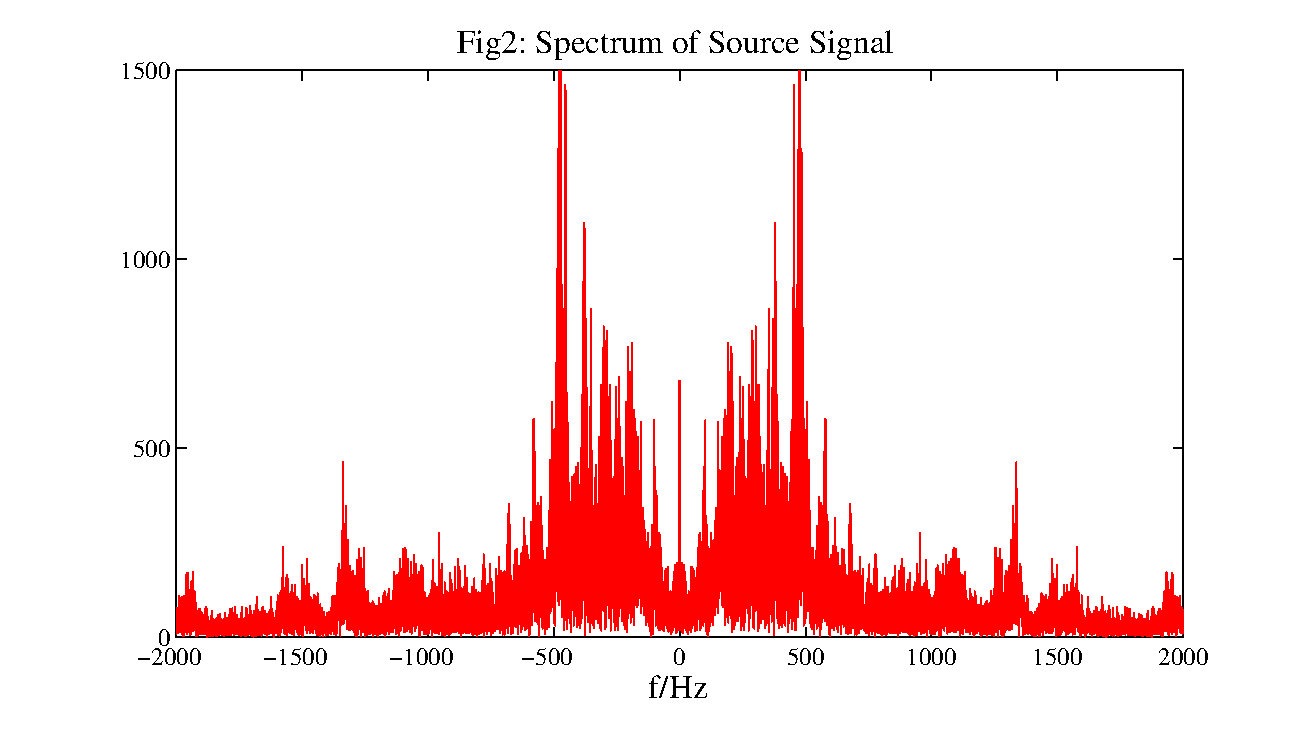
\includegraphics[width=1\textwidth]{fig2.eps}
\end{center}

\subsection{加高斯白噪声}
对于已经录制好的源信号,为其添加信噪比确定的高斯白噪声,来模拟真实信道传输特性。在试验中,令信噪比为$SNR = 5dB$,得到加噪声后的信号的时域波形和频谱图分别如图3和图4所示。
\begin{center}
    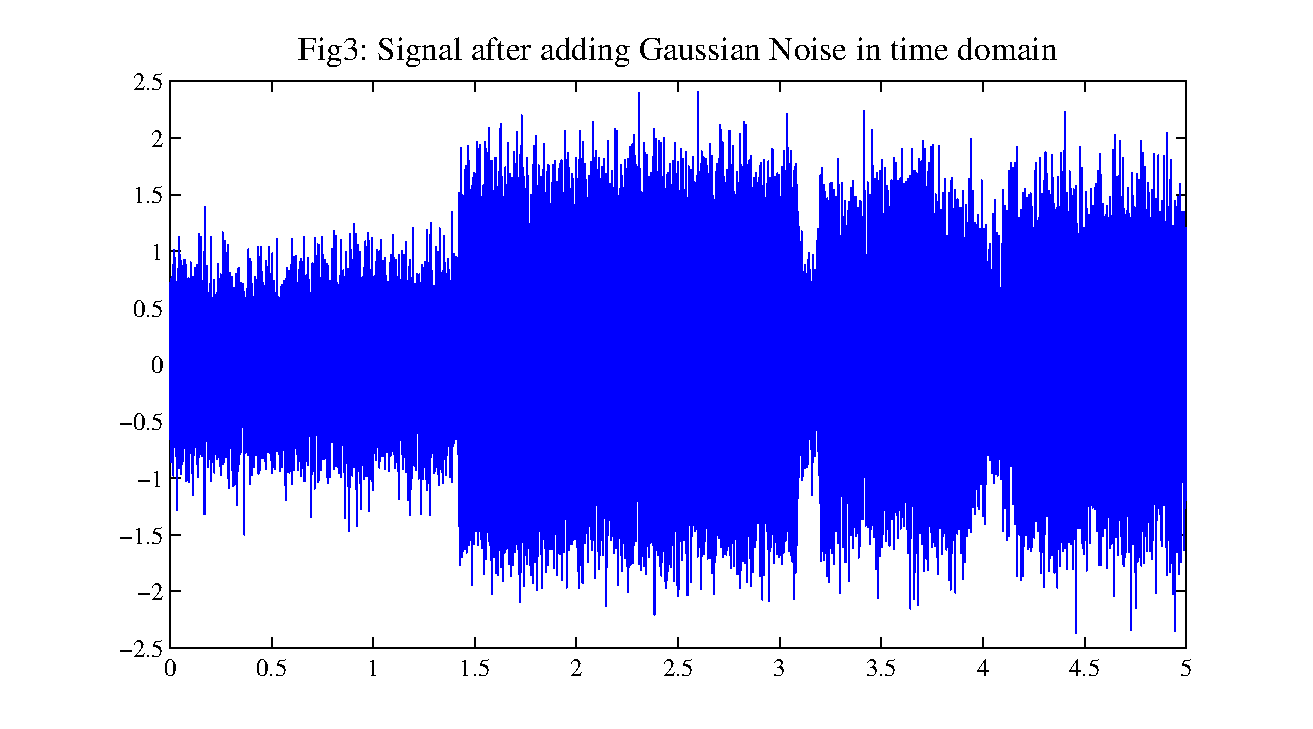
\includegraphics[width=1\textwidth]{fig3.eps}
\end{center}
\begin{center}
    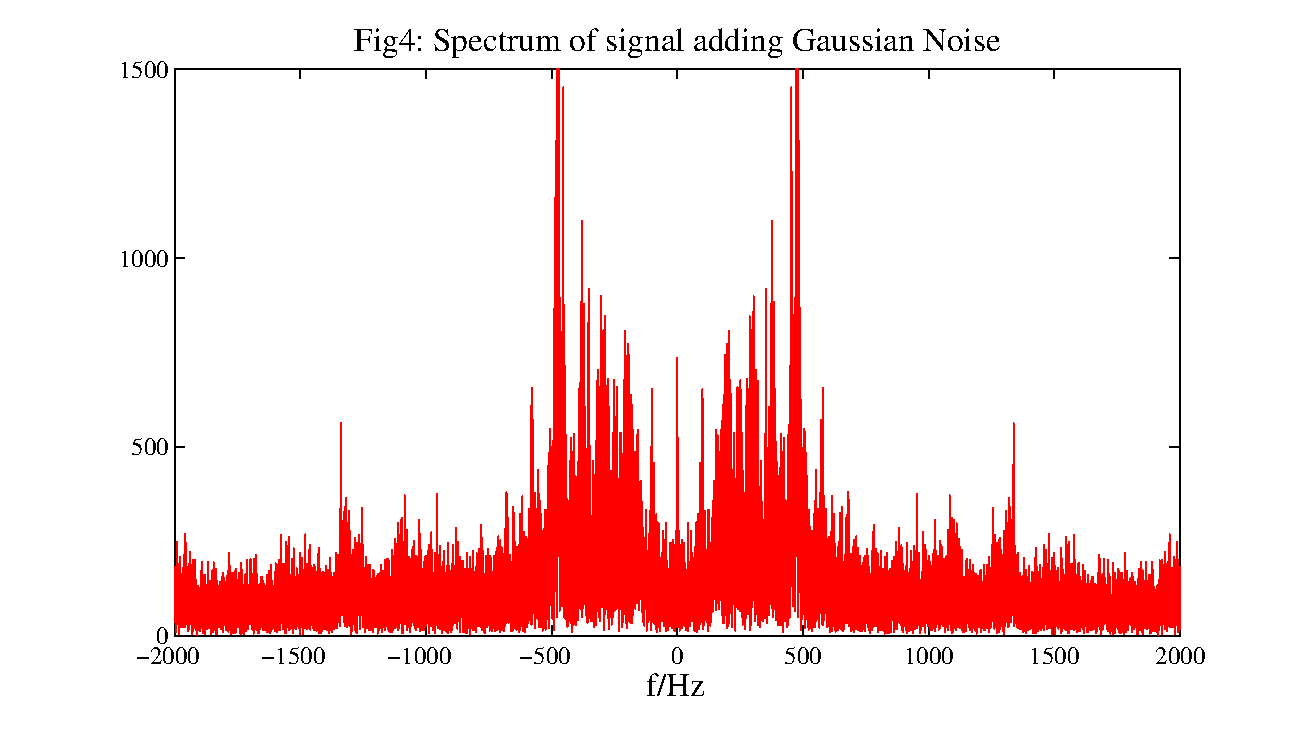
\includegraphics[width=1\textwidth]{fig4.eps}
\end{center}

对比加噪声前后的时域图,可以清晰地发现噪声使得信号的幅度更加均匀,并且边界上有更多的毛刺。而对比两个频谱图也可以看到加噪声后各个频谱分量都有所增加。鉴于人的声音频率范围大约是85$Hz$$\sim$1100$Hz$之间,并且考虑到笔者为男生,声音更加低沉,设计指标则初步定为滤除高频的杂音分量。

\subsection{滤波器设计}
本节中,笔者分别用上述两种映射方法以及基于两种不同的模拟原型滤波器~(切比雪夫$I$和巴特沃斯),设计了2种滤波器。接下来分别阐述设计过程和实验现象。

\subsubsection{设计指标}
在介绍不同滤波器前,首先明确本次设计的最终指标。从图4中可以看到,在$f=500Hz$点上有明显的频率分量~(归一化功率最大),且当频率再增加,会有不同幅度的高频分量。鉴于此,为了更加明显的看到滤波器的滤波效果,设计指标定为:
\begin{enumerate}
\item 抽样频率$8kHz$,数字低通滤波器;
\item 通带上限$300Hz$, 阻带临界$500Hz$~(最终结果应能看到$f=500Hz$点的变化);
\item 通带最大衰减$1dB$,阻带最小衰减$50dB$。
\end{enumerate}

\subsubsection{方法1:脉冲响应不变法设计低通切比雪夫I型}
首先,笔者采用脉冲响应不变法来设计低通切比雪夫I型滤波器。对于已有的设计指标,需要先转化为模拟域上的设计指标,之后进行阶数$N$ 和截止频率$\Omega_c$的计算。这样我们得到了归一化的低通滤波器,之后通过去归一化来得到模拟滤波器的传递函数。最后,通过脉冲响应不变法转换为数字滤波器传递函数,得到设计结果。部分$Matlab$代码如下:

% ===================================插入Matlab代码格式,参考matlab-prettifier文档
\begin{lstlisting}[style=Matlab-editor,
                   basicstyle=\mlttfamily,
                   caption={Designing IIR Filter Code}, label=code1]
wp = 2*pi*300;
ws = 2*pi*500;      %  数字滤波器特征转化到模拟滤波器频率特征
Rp = 1;
Rs = 50;
Fs = 8000;
[N, Wn] = cheb1ord(wp,ws,Rp,Rs,'s');        %  选择滤波器的最小阶数
[Z, P, K] = cheb1ap(N,Rp);                  %  创建低通切比雪夫I滤波器
[A, B, C, D] = zp2ss(Z,P,K);                %  归一化低通滤波器
[At, Bt, Ct, Dt] = lp2lp(A,B,C,D,Wn);       %  去归一化,得到截止频率 Wn 的
[num_ana,den_ana] = ss2tf(At,Bt,Ct,Dt);     %  得到模拟滤波器传递函数(分子、分母多项式系数)
[num_dig,den_dig] = impinvar(num_ana,den_ana,Fs);      %  脉冲响应不变法 转换为数字滤波器传递函数(分子、分母多项式系数)
\end{lstlisting}

其中,代码可以在运行过程中给出设计滤波器的零、极点数值。这里给出滤波器系统函数的分子分母多项式系数,分别为:

\vspace{0.2cm}
\begin{center}
\begin{tabular}{|l|l|l|l|}
  \hline
  \multirow{8}{2cm}{b = $10^{-6}$ $\ast$}
                & 0.0000 &
  \multirow{8}{2cm}{a = $10^{-6}$ $\ast$} & 1.0000\\
                & 0.0017 &  & -6.6877\\
                & 0.0915 &  & 19.2639\\
                & 0.4689 &  & -30.9784\\
                & 0.4545 &  & 30.0341\\
                & 0.0834 &  & -17.5544\\
                & 0.0014 &  & 5.7271\\
                & 0.0000 &  & -0.8045\\
  \hline
\end{tabular}
\end{center}
\vspace{0.2cm}

生成的低通切比雪夫I型的幅频响应如图5所示。在图中可以看到当频率$f\leq 300Hz$时,幅度平方函数不衰减;而当频率$f=500Hz$时,其衰减为$55dB\ge 50dB$,说明满足设计要求。对于切比雪夫滤波器,可以看到其通带内是等波纹的。
\begin{center}
    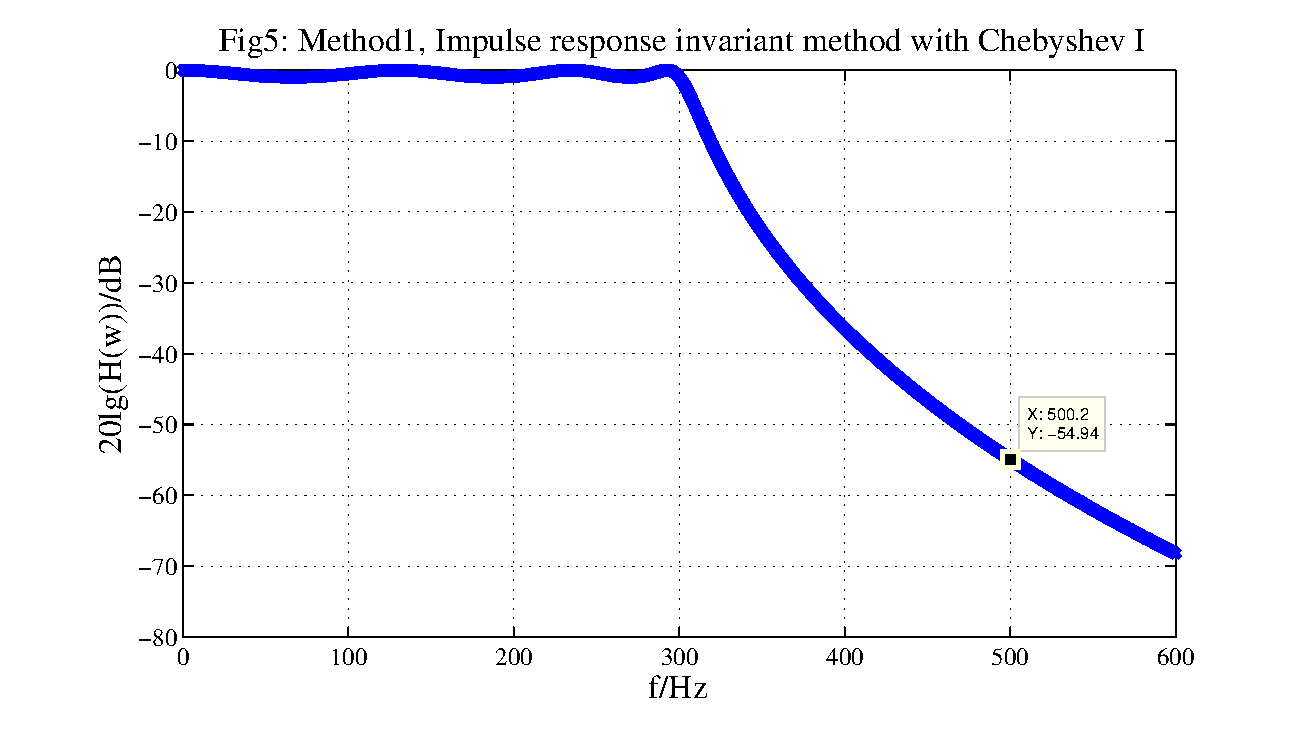
\includegraphics[width=1\textwidth]{fig5.eps}
\end{center}

在图6中,我们画出了此切比雪夫I型低通滤波器的相频响应和零极点分布图。在左子图中我们可以看到其相频响应不是线性的,这是IIR的特点所造成的,在之后会进行详细分析。而零极点图也符合我们的预期,每一个零、极点都在单位圆内,说明此系统是稳定的。
\begin{center}
    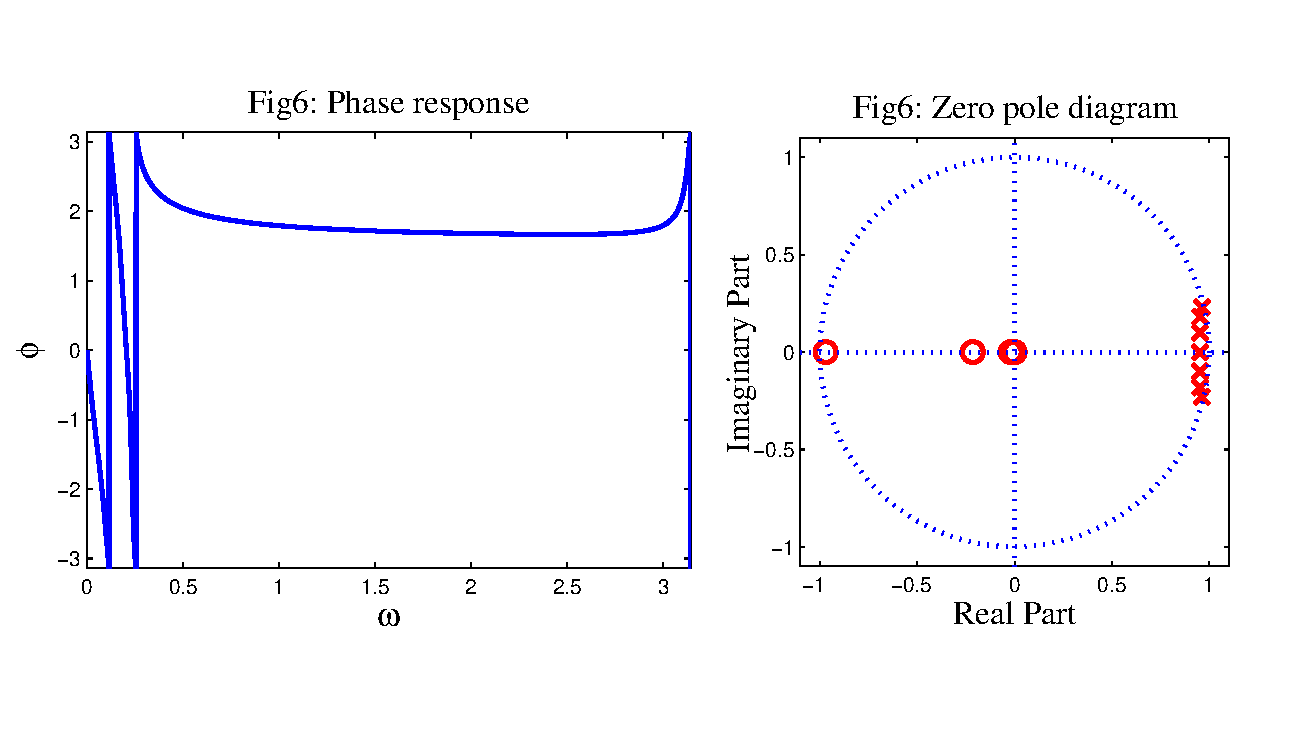
\includegraphics[width=1\textwidth]{fig6.eps}
\end{center}

图7中,我们给出了加噪声的源信号通过此切比雪夫低通滤波器后的频谱图。由图可见在通带外,即$f>500Hz$时是完全没有信号通过的,而在过渡带也有一个明显的衰减。具体的讨论对于在下一章节中详细说明。
\begin{center}
    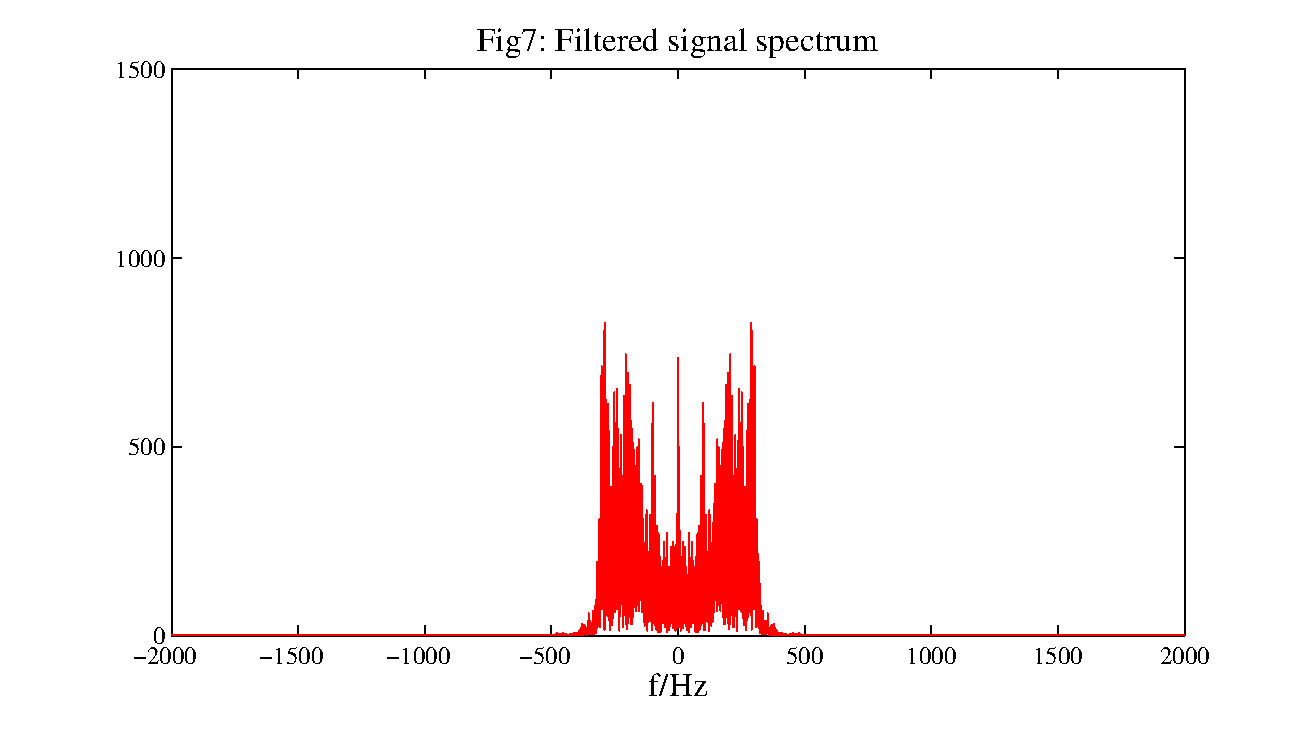
\includegraphics[width=1\textwidth]{fig7.eps}
\end{center}

\subsubsection{方法2:双线性变换法设计低通巴特沃斯}
在用脉冲响应不变法设计后,笔者尝试用另一种方法,即双线性变换法来设计低通滤波器,指标与之前相同。为了体现设计过程的不同,此次选择的原型滤波器是巴特沃斯滤波器。在下一章节,会对两种不同滤波器的滤波效果进行对比。

设计流程大体和之前一样,主要是对应的映射关系不同,这里不再赘述。部分关键的$Matlab$代码如下:

% ===================================插入Matlab代码格式,参考matlab-prettifier文档
\begin{lstlisting}[style=Matlab-editor,
                   basicstyle=\mlttfamily,
                   caption={Designing IIR Filter Code}, label=code2]
Wp = 0.075*pi;            %  通带边界频率(归一化):wp=fp*2*pi/fs
Ws = 0.125*pi;            %  阻带边界频率(归一化):ws=fr*2*pi/fs
Rp = 1;                   %  通带波纹
Rs = 50;                  %  阻带衰减
Ts = 0.000125;            %  Fs = 8kHz
%   转换为模拟滤波器指标(预畸变)
OmegaP = (2/Ts)*tan(Wp/2);        %  模拟低通原型滤波器通带频率
OmegaS = (2/Ts)*tan(Ws/2);        %  模拟低通原型滤波器阻带频率
[N, OmegaC] = buttord(OmegaP,OmegaS,Rp,Rs,'s');     %  模拟巴特沃斯滤波器的阶数和-3dB截止频率计算
[Z, P, K] = buttap(N);                              %  设计归一化巴特沃兹滤波器低通原型
num_ana = K * real(poly(Z));
den_ana = real(poly(P));                            %  原型(归一化)滤波器系数
[num_ana, den_ana] = lp2lp(num_ana,den_ana,OmegaC); %  去归一化处理,得到截止频率 OmegaC 的
[num_dig, den_dig] = bilinear(num_ana,den_ana,Fs);  %  双线性变换法 转换为数字滤波器传递函数
\end{lstlisting}

其中,代码同样可以在运行过程中给出设计滤波器的零、极点数值。这里给出滤波器系统函数的分子分母多项式系数,分别为:

\vspace{0.2cm}
\begin{center}
\begin{tabular}{|l|l|l|l|}
  \hline
  \multirow{14}{2cm}{b = $10^{-8}$ $\ast$}
                & 0.0001 &
  \multirow{14}{2cm}{a = $10^{-8}$ $\ast$} & 1.0000\\
                & 0.0011 &  & -10.8920\\
                & 0.0065 &  & 54.9026\\
                & 0.0240 &  & -169.5601\\
                & 0.0598 &  & 357.9343\\
                & 0.1080 &  & -545.3253\\
                & 0.1436 &  & 616.8462\\
                & 0.1440 &  & -524.4779\\
                & 0.1077 &  & 335.1767\\
                & 0.0600 &  & -158.9978\\
                & 0.0239 &  & 54.4147\\
                & 0.0065 &  & -12.7221\\
                & 0.0011 &  & 1.8211\\
                & 0.0001 &  & -0.1205\\
  \hline
\end{tabular}
\end{center}
\vspace{0.2cm}

生成的低通巴特沃斯滤波器的幅频响应如图8所示。在图中可以看到当频率$f\leq 300Hz$时,幅度平方函数不衰减;而当频率$f=500Hz$时,其衰减约高于$50dB$,说明满足设计要求。此设计结果对比切比雪夫滤波器,可以看出其通带内是平滑的,单调下降形式。
\begin{center}
    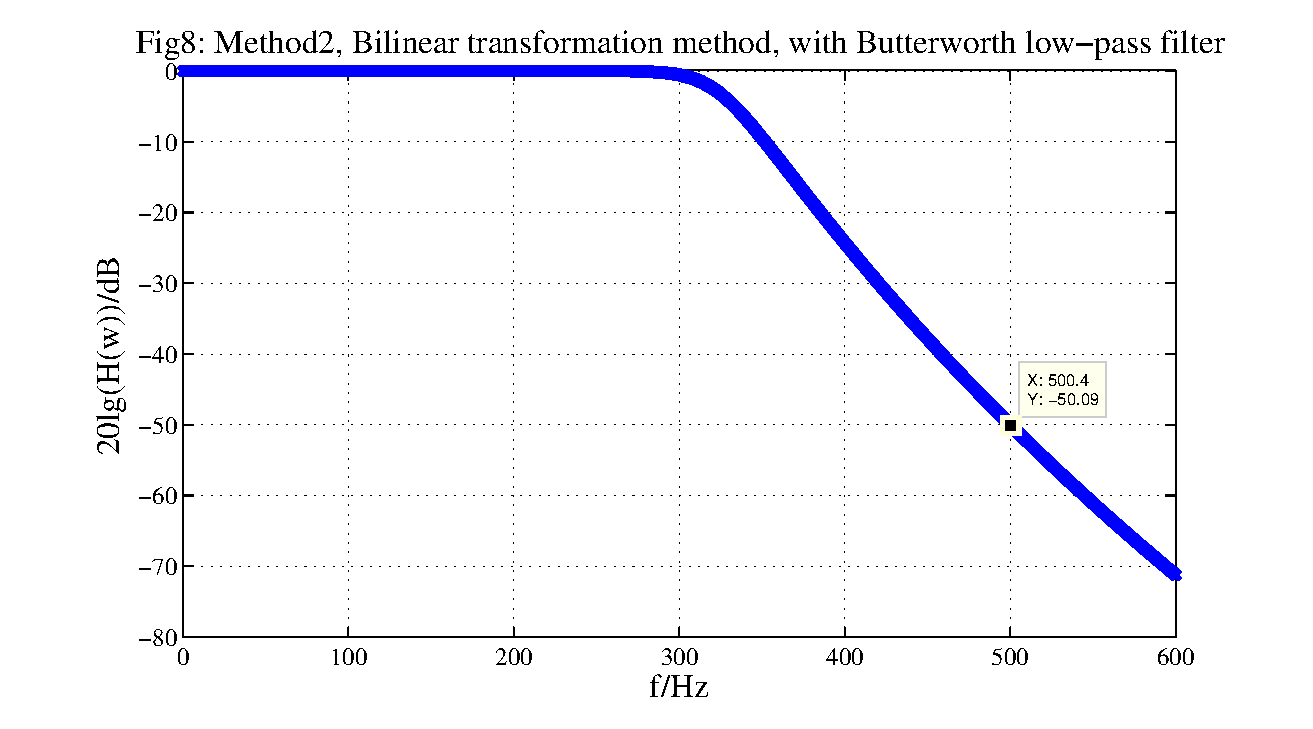
\includegraphics[width=1\textwidth]{fig8.eps}
\end{center}

在图9中,我给出此巴特沃斯低通滤波器的相频响应和零极点分布图。在左子图中我们可以看到其相频响应不是线性的,而对比利用脉冲响应不变法的结果,可以看出这里的分线性更加明显,这是由双线性变换法的固有特性造成的,之后进行讨论。而零极点图也同样符合预期,每一个极点都在单位圆内,说明此系统是稳定的;而零极点的出现也分别是共轭的。
\begin{center}
    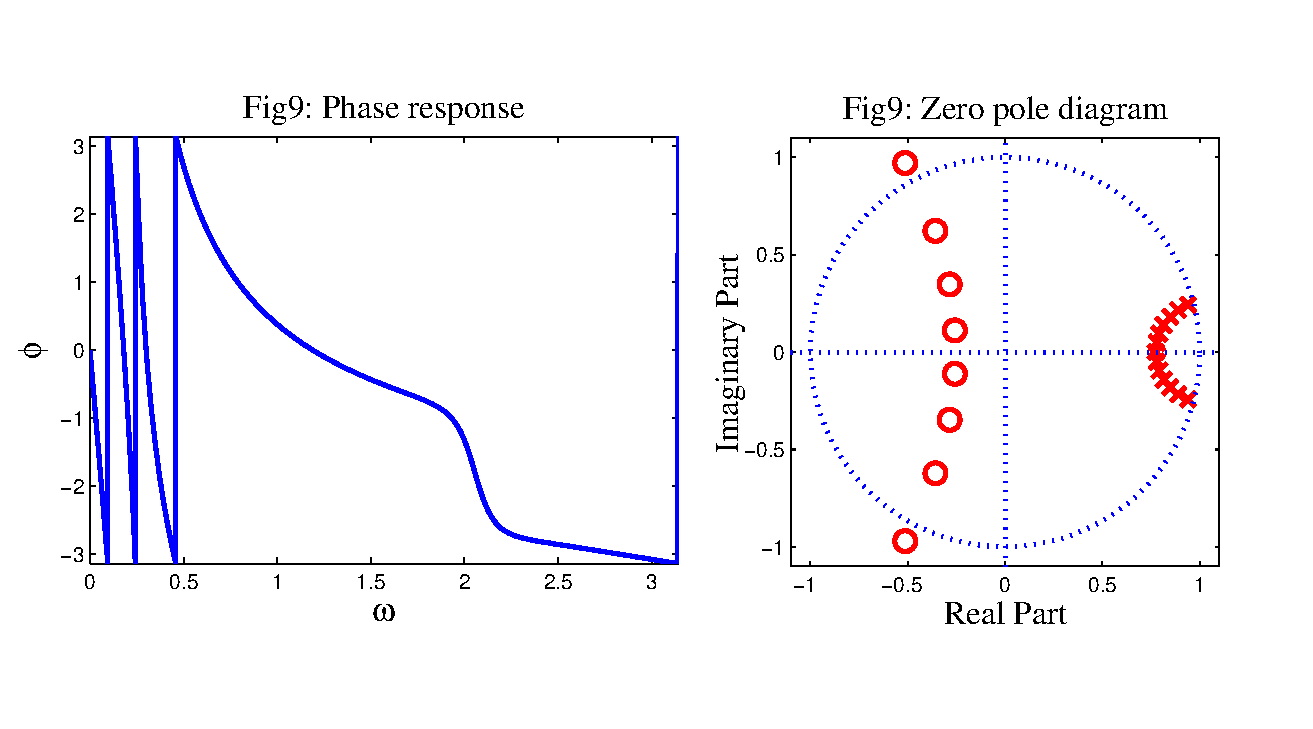
\includegraphics[width=1\textwidth]{fig9.eps}
\end{center}

最后在图10中,我们给出了加噪声后的源信号通过此巴特沃斯滤波器后的频谱图。此频谱图与图7类似,均能较好的滤除带外的信号而保留带内的信号;有所不同的地方是在过渡带内的表现,在下一节中进行讨论。
\begin{center}
    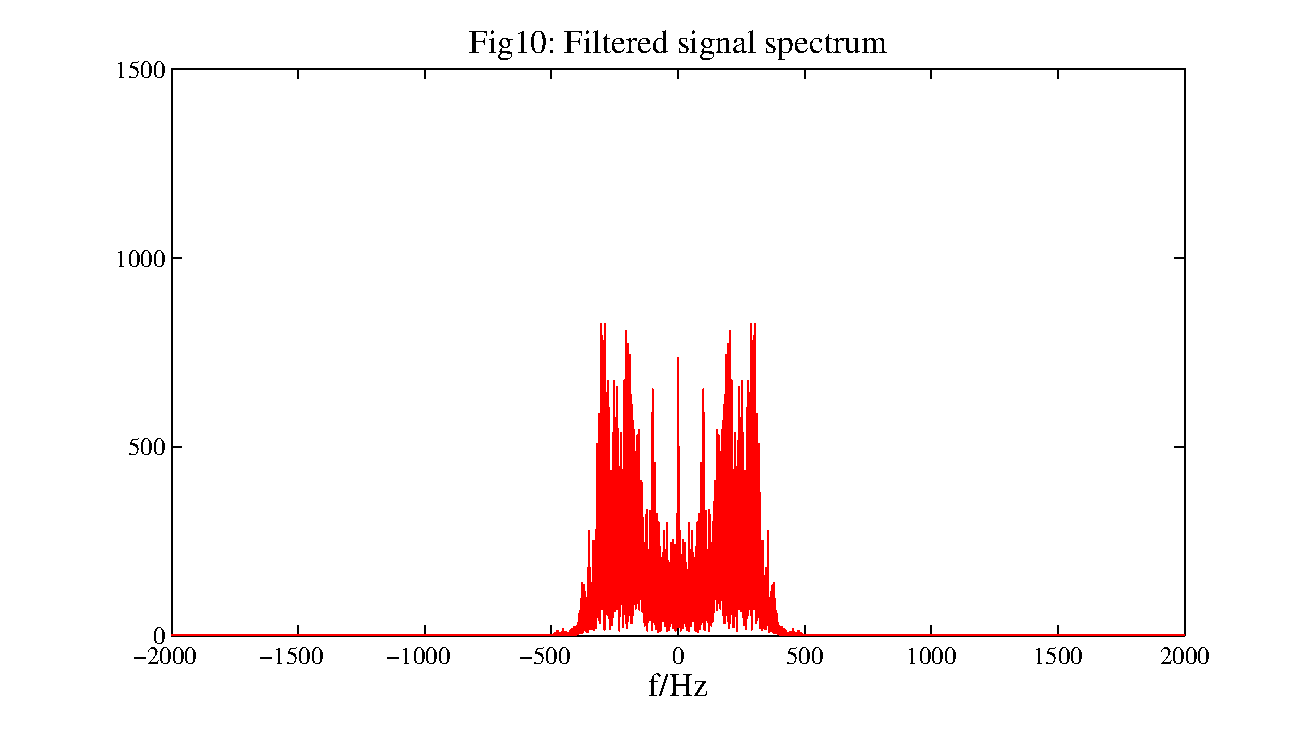
\includegraphics[width=1\textwidth]{fig10.eps}
\end{center}


\section{实验结果分析}

\subsection{方法1:脉冲响应不变法设计低通切比雪夫I型}
对于切比雪夫I型滤波器,其通带内是等波纹的,即I型幅频特性在通带内等波纹,在阻带内单调下降。从图中的标记处可以看到,在阻带边界频率$f=500Hz$上,其幅度平方函数的衰减为$54.94dB$,比预计的$50dB$要好,而同样指标的巴特沃斯滤波器只是刚刚达到标准,这是由于保证通带边缘满足设计指标,在通带内有很大裕量可能是一种浪费,切比雪夫滤波器通过允许通带上的波纹使得衰减更加迅速。

而对于相频函数,由于IIR滤波器本身的结构具有强反馈的特征,相位上的一点点延迟在经过多级反馈之后都会被放大许多,导致出现非线性。

最后,当源信号通过此滤波器时,在原频谱上的``最大分量'',即$f=500Hz$频点的响应,可以看到已经完全滤掉。这样是将源声音信号的高频分量滤掉,并且可以看到在过渡带~($300\sim 500Hz$)中,其下降的趋势也非常陡,说明了设计的滤波器的功能是超过预期指标的。

\subsection{方法2:双线性变换法设计低通巴特沃斯}
对于巴特沃斯滤波器,其在整个带宽内都是严格下降的,从图8中我们也可以看到在阻带边界频率$f=500Hz$上,其幅度平方函数的衰减也仅仅是略微大于$50dB$,比起同样设计条件的切比雪夫I型滤波器要差一点,这也是因为通带内有很大裕量可能是一种浪费造成的,不再多加赘述。

对于其相位谱而言,在阻带内对比切比雪夫I型滤波,可以从图9看出存在较大的非线性,这是因为:
\begin{equation}
\Omega = c \tan (\frac{\Omega_1 T}{2}) = c \tan (\frac{\omega}{2}).
\end{equation}

当条件满足$\Omega_1 = \omega \/ T$较小时,可以得到
\begin{equation}
\Omega = c \tan (\frac{\Omega_1 T}{2}) \thickapprox c \frac{\Omega_1 T}{2},
\end{equation}
可以推出在低频范围内,存在近似:
\begin{equation}
c \thickapprox \frac{2}{T}.
\end{equation}

即对于常数$c$的取值,于抽样间隔时间$T$相关。但是对于高频分量而言,这种近似不成立,而又由于双线性变换法的非线性映射,造成了高频分量的相位谱出现严重的非线性,这也在图9中有明显的体现。

最后,当源信号通过此巴特沃斯滤波器时,在原频谱上的``最大分量''$f=500Hz$频点的响应已经完全滤掉,这和之前的切比雪夫的结果是一样的。在过渡带~($300\sim 500Hz$)中,其下降的趋势比较陡,但是表现没有同等条件下切比雪夫的要好,这也说明了切比雪夫的下降是更迅速的。

综上,两个设计的滤波器都达到了预期的设计指标,都能很好的滤除带外的信号分量,而保留所需要的频率分量。对于过渡带内的衰减,则是有原型模拟滤波器的参数特性所决定,在实验中可以看出是切比雪夫表现更好。本实验最后的结论也说明了两个IIR滤波器设计的正确性,以及对源信号的分量提取的有效性。

\section{总结}
本次报告对关于IIR数字滤波器的基础知识和设计内容做了介绍,完整且超额完成了实验过程,并给出了实验过程数据图,最后作出了详细的结果分析。经过本次实验,本人对IIR数字滤波器的设计有了更深的理解,并对较晦涩难懂的内容,例如频率在不同域的互相转换,梳理得更加清楚。本次实验也让我认识到了自己的不足之处,对给出的问题需要思考整理较久思路,之后还要多加注意。


\section{附录}
$Matlab$代码的使用是添至搜索路径运行即可,注意其中是``load''了已存好的$.mat$文件,录音部分被注释掉~(要是重新录制只需要注释掉``load''语句即可)。

本文的图片均为$.eps$格式,可以进行缩放而不失真的矢量图,在观察某些细节(例如滤波器响应等)时观察得更清楚。由于$Matlab$ 含有中文的图片在导出$.eps$文件时会出现乱码情况,故所有图片的标题等均为英文所写。

最后,由于报告中需要加入许多数学表达式,本文档使用了$LaTeX$来编写报告,以获得更优的排版效果。
\iffalse
\footnote{由于另一篇文章《学习心得与体会》我写的较为全面,涵盖了这部分的内容,所以两篇文章会有部分内容是一样的,但均为自己构思、写出的,可视作对前部分内容的加深、拓展。}。
\fi


% =====================================================Reference
\small
\begin{thebibliography}{99}
\setlength{\parskip}{0pt}  %段落之间的竖直距离

\bibitem{wiki}
https://zh.wikipedia.org/wiki.

\bibitem{textbook}
程佩青. 数字信号处理教程~(第三版), 清华大学出版社, 2012.6.

\bibitem{wikifft}
Brenner, N.; Rader, C. A New Principle for Fast Fourier Transformation. \emph{IEEE Acoustics, Speech \& Signal Processing}. 1976, 24(3): 264–266.

\bibitem{course1}
程宇新. 第4章, 滤波器概要, 数字滤波器结构1, IIR结构. 2017, 4.

\bibitem{course2}
程宇新. 第5章, IIR滤波器设计, 从模拟滤波器到数字滤波器. 2017, 5.

\bibitem{course3}
程宇新. 第5章, IIR滤波器设计, 模拟滤波器设计. 2017, 5.

\bibitem{course4}
程宇新. 第5章, IIR滤波器设计, 频率变换法. 2017, 5.

\bibitem{ta}
TA. 数字信号处理第二次上机. 2017, 5.

\end{thebibliography}

\clearpage
\end{document}
